% Diagram 4.4.4: preserve both components, the deleted point and the red images.
\begin{tikzcd}[column sep=large,row sep=1.8em]
R=(\mathbb Z/2\times\mathbb A^1)\setminus\{(-1,0)\}\arrow[d]&
{\begin{tikzpicture}[baseline=-3pt,x=1cm,y=1cm,font=\small]
\draw[line width=.7pt] (-1.65,.22)--(1.65,.22);
\draw[line width=.7pt] (-1.65,0)--(1.65,0);
\fill[white] (0,0) circle (2.1pt);
\draw (0,0) circle (2.1pt);
\fill[red] (.9,0) circle (2pt);
\node[red,below] at (.9,0) {$x$};
\node[red,anchor=west] (unit) at (1.7,.55) {单位截面};
\draw[red,->] (unit.west)--(1.62,.24);
\end{tikzpicture}}\arrow[d,shift right=3pt,"p_2"']\arrow[d,shift left=3pt,"\sigma"]\\
\mathbb A^1&
{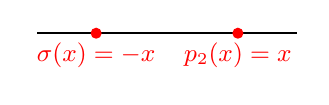
\begin{tikzpicture}[baseline=-3pt,x=1cm,y=1cm,font=\small]
\draw[line width=.7pt] (-1.65,0)--(1.65,0);
\fill[red] (-.9,0) circle (2pt);
\fill[red] (.9,0) circle (2pt);
\node[red,below] at (-.9,0) {$\sigma(x)=-x$};
\node[red,below] at (.9,0) {$p_2(x)=x$};
\end{tikzpicture}}
\end{tikzcd}
